% Figure snippet: baseline levels + relIns version for full audits
% Requires tablenotes support in your preamble/template.

\begin{figure}[H]
    \centering
    \caption{Effort Response to Audit Success, Algorithm-Selected Full Audits}
    \label{fig:effortresponse-scatter-levels}
    \begin{tabular}{cc}
    \multicolumn{2}{c}{A: Share of Void Cases} \\
    A1: 2018 vs 2019     &  A2: 2018 vs 2019-2020 average\\
    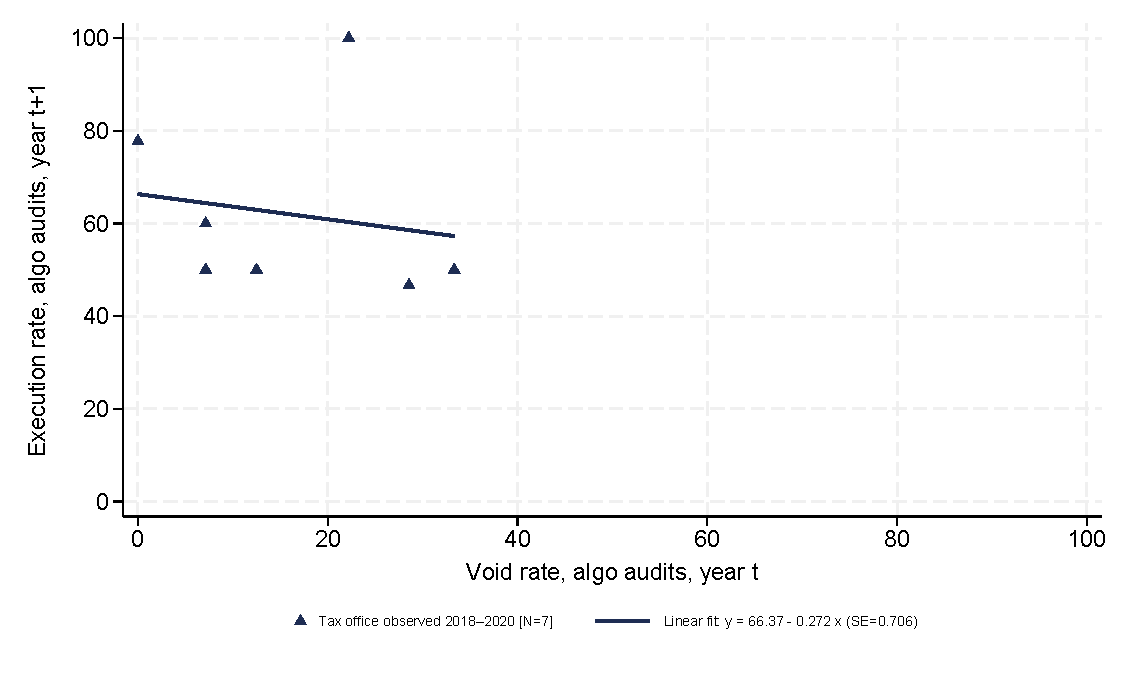
\includegraphics[width=0.5\linewidth]{Output/scatter_share_v_Algorithm_2018_2019_full.pdf}  &  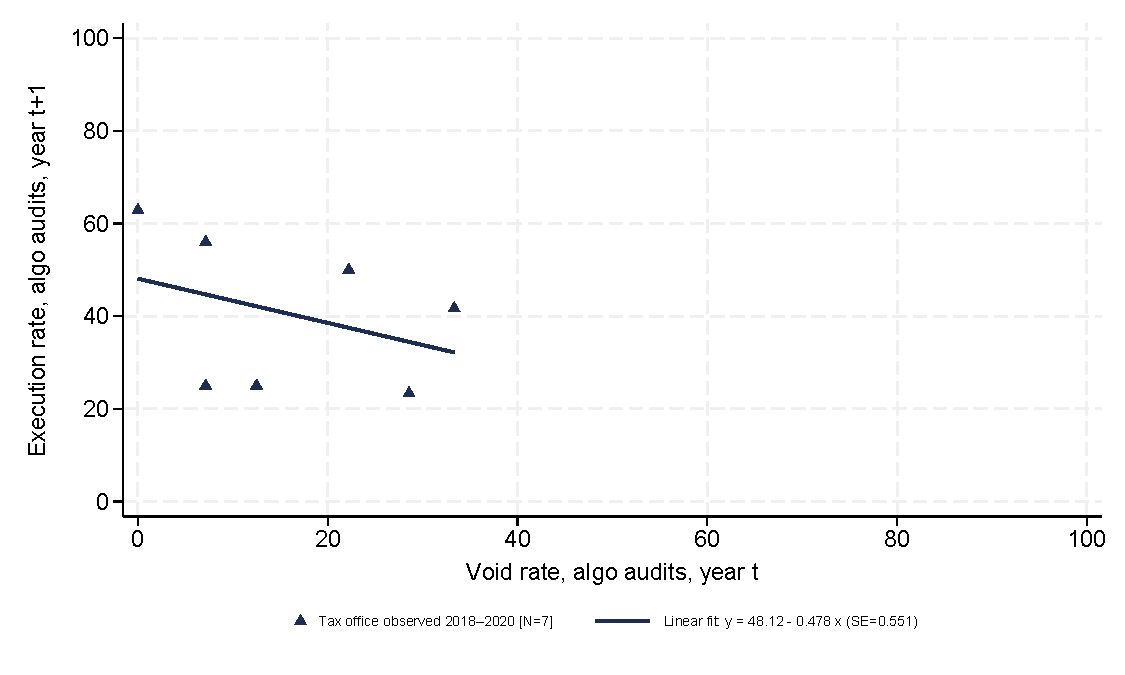
\includegraphics[width=0.5\linewidth]{Output/scatter_share_v_Algorithm_2018_avg_full.pdf} \\
    \multicolumn{2}{c}{B: Below-Median Evasion Rate} \\
    B1: 2018 vs 2019     &  B2: 2018 vs 2019-2020 average\\
    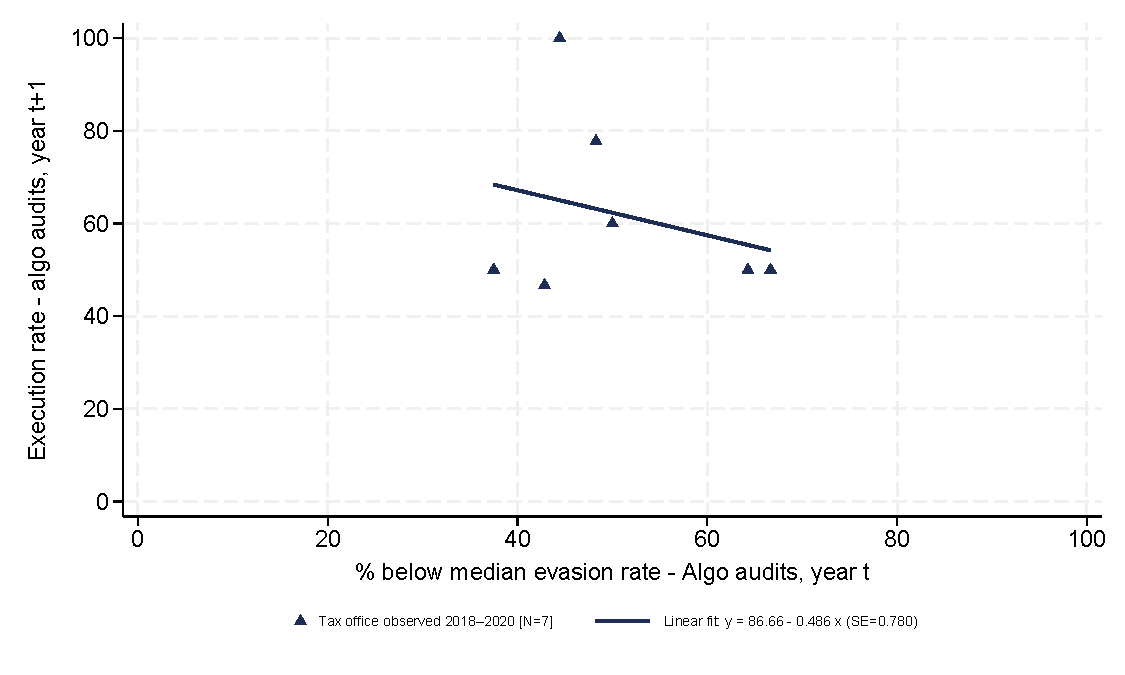
\includegraphics[width=0.5\linewidth]{Output/scatter_share_med_er_Algorithm_2018_2019_full.pdf}  &  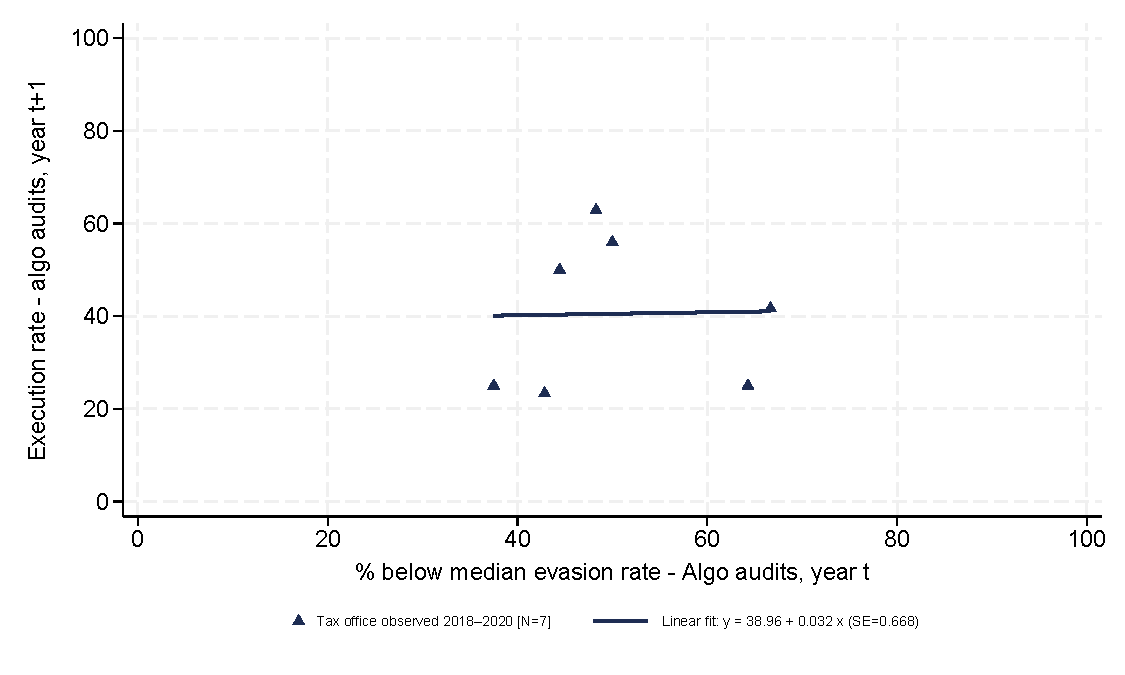
\includegraphics[width=0.5\linewidth]{Output/scatter_share_med_er_Algorithm_2018_avg_full.pdf} \\
    \multicolumn{2}{c}{C: Bottom-Quartile Evasion Rate} \\
    C1: 2018 vs 2019     &  C2: 2018 vs 2019-2020 average\\
    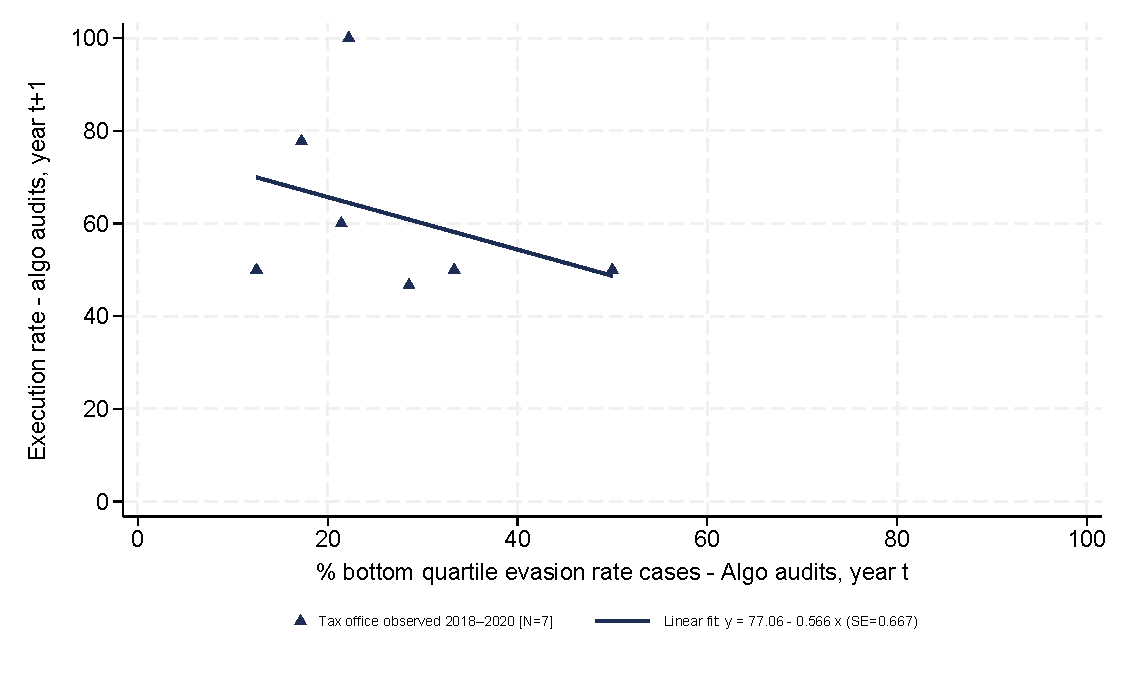
\includegraphics[width=0.5\linewidth]{Output/scatter_share_botq_er_Algorithm_2018_2019_full.pdf} &
    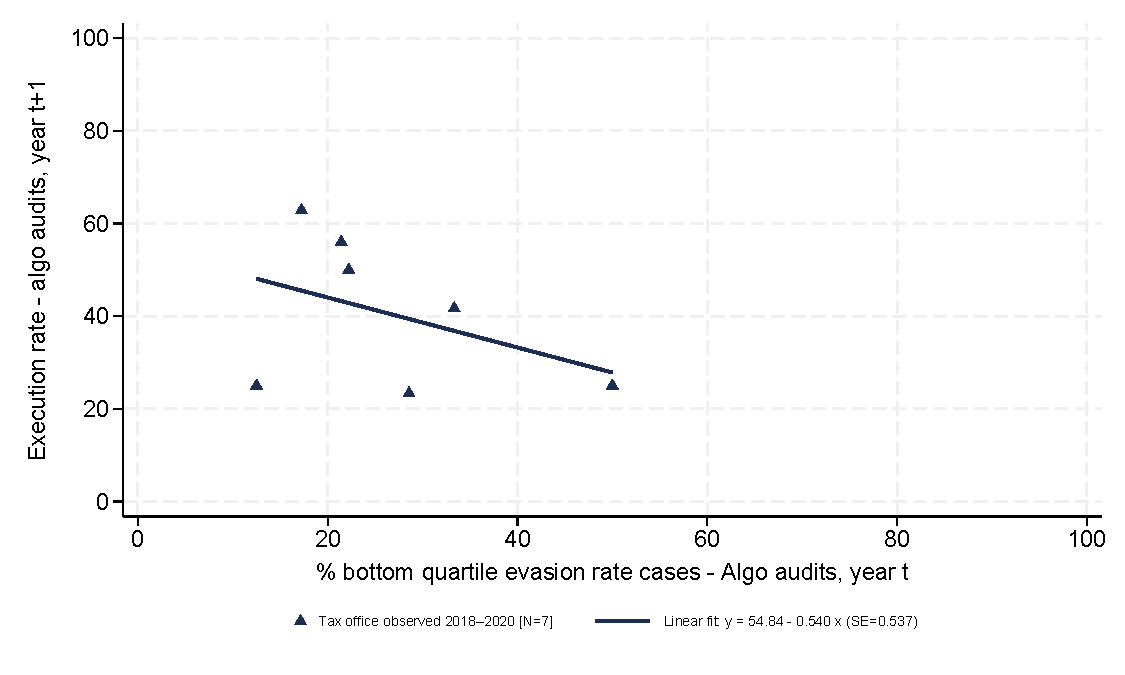
\includegraphics[width=0.5\linewidth]{Output/scatter_share_botq_er_Algorithm_2018_avg_full.pdf}   \\
    \end{tabular}
    \begin{tablenotes}
    \footnotesize \item Notes: The sample is restricted to selected full audits, excluding safety cases. Observations are aggregated at the tax-office-year level. For method \(m \in \{\text{Algorithm}, \text{Inspectors}\}\), the void share is \(\text{null evasion}_m / \text{executed}_m\); the below-median and bottom-quartile evasion-rate shares are defined analogously using method-specific executed audits; and the execution rate is \(\text{executed}_m / \text{assigned}_m\). Panels A--C plot the Algorithm share in year \(t\) (x-axis) against the Algorithm execution rate in \(t+1\) (y-axis), where \(t+1\) is either 2019 or \(\text{avg}(2019,2020)\). The \(\text{avg}(2019,2020)\) term is computed as the row mean of 2019 and 2020 values. Points are unweighted office-year observations. Solid and dashed lines are separate unweighted OLS fits by office-coverage group.
    \end{tablenotes}
\end{figure}

\begin{figure}[H]
    \centering
    \caption{Effort Response to Audit Success, Algorithm-Selected Full Audits (Relative to Inspector Selection)}
    \label{fig:effortresponse-scatter-relins}
    \begin{tabular}{cc}
    \multicolumn{2}{c}{A: Share of Void Cases (Algorithm / Inspectors)} \\
    A1: 2018 vs 2019     &  A2: 2018 vs 2019-2020 average\\
    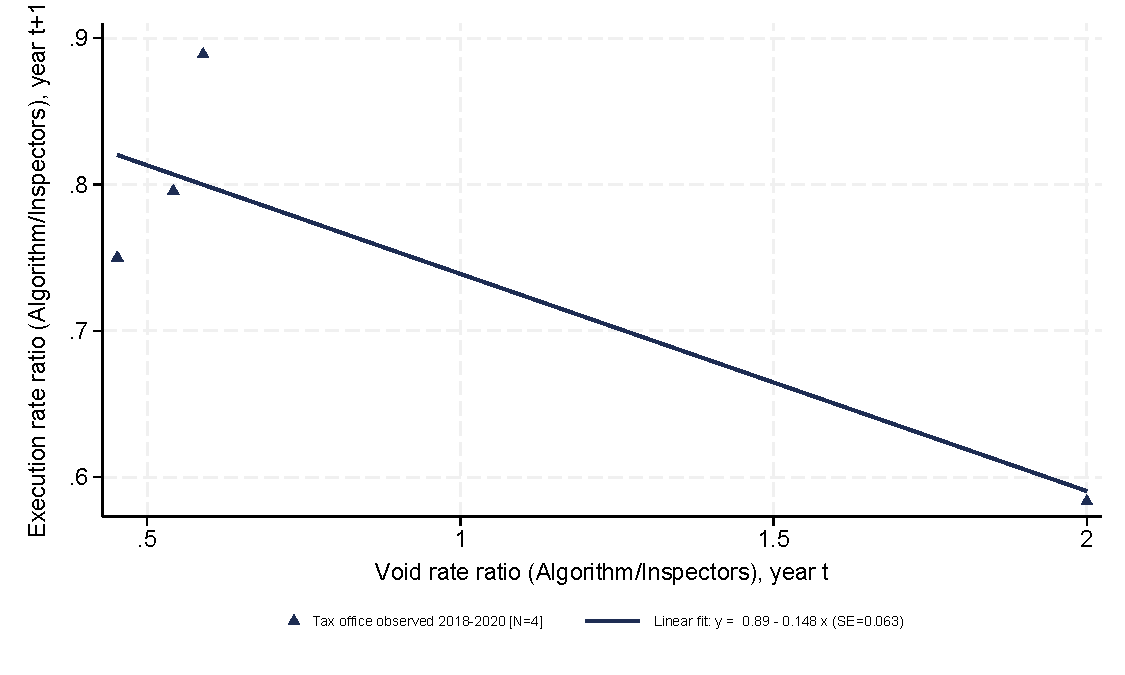
\includegraphics[width=0.5\linewidth]{Output/scatter_share_v_relIns_Algorithm_2018_2019_full.pdf}  &
    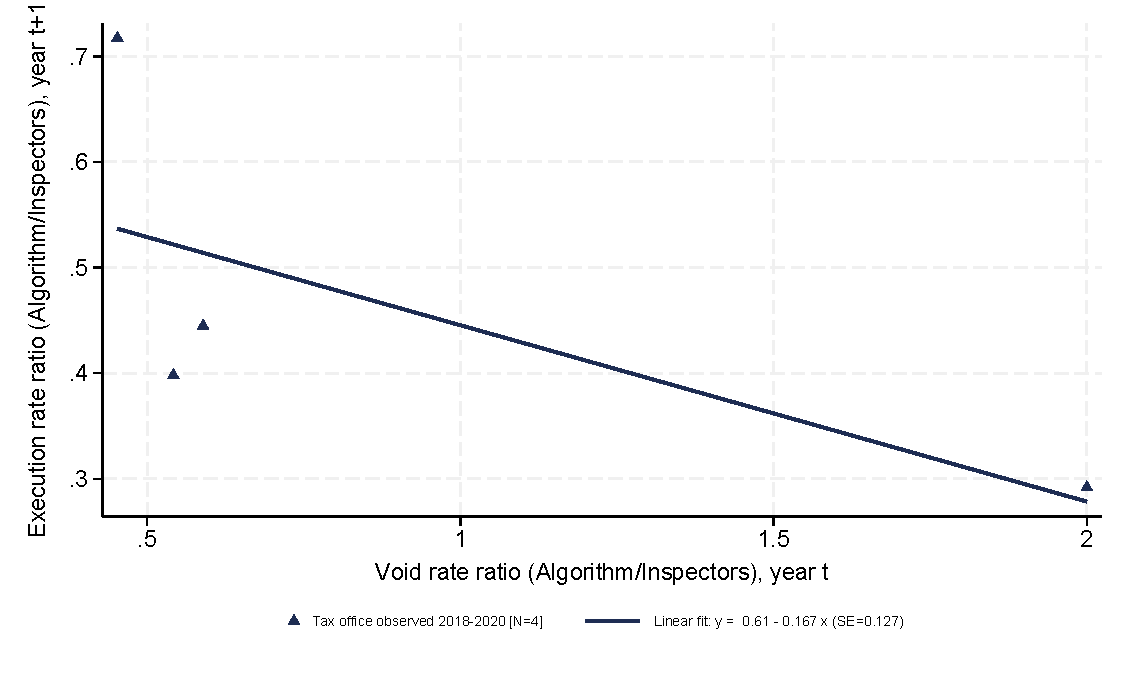
\includegraphics[width=0.5\linewidth]{Output/scatter_share_v_relIns_Algorithm_2018_avg_full.pdf} \\
    \multicolumn{2}{c}{B: Below-Median Evasion Rate (Algorithm / Inspectors)} \\
    B1: 2018 vs 2019     &  B2: 2018 vs 2019-2020 average\\
    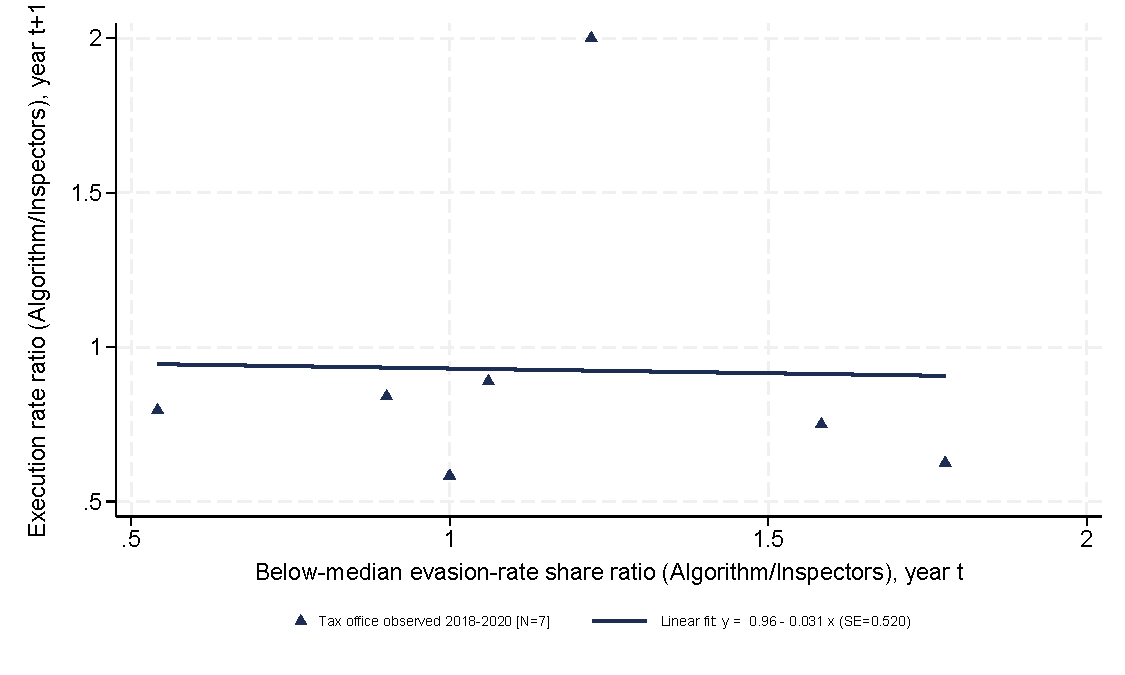
\includegraphics[width=0.5\linewidth]{Output/scatter_share_med_er_relIns_Algorithm_2018_2019_full.pdf}  &
    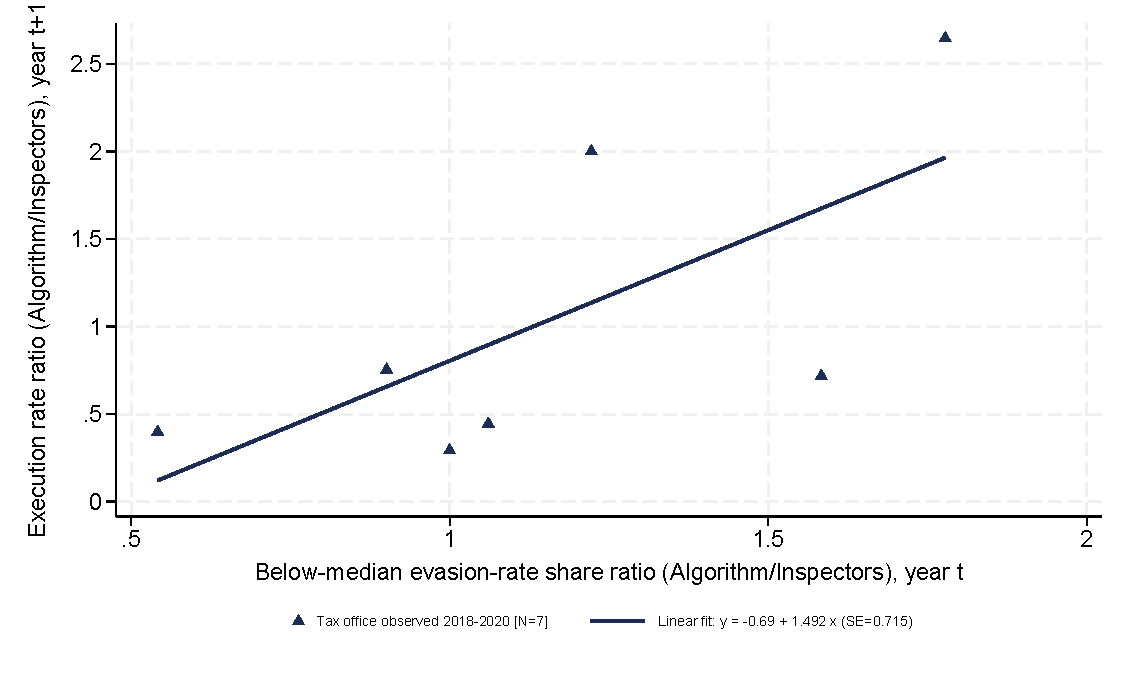
\includegraphics[width=0.5\linewidth]{Output/scatter_share_med_er_relIns_Algorithm_2018_avg_full.pdf} \\
    \multicolumn{2}{c}{C: Bottom-Quartile Evasion Rate (Algorithm / Inspectors)} \\
    C1: 2018 vs 2019     &  C2: 2018 vs 2019-2020 average\\
    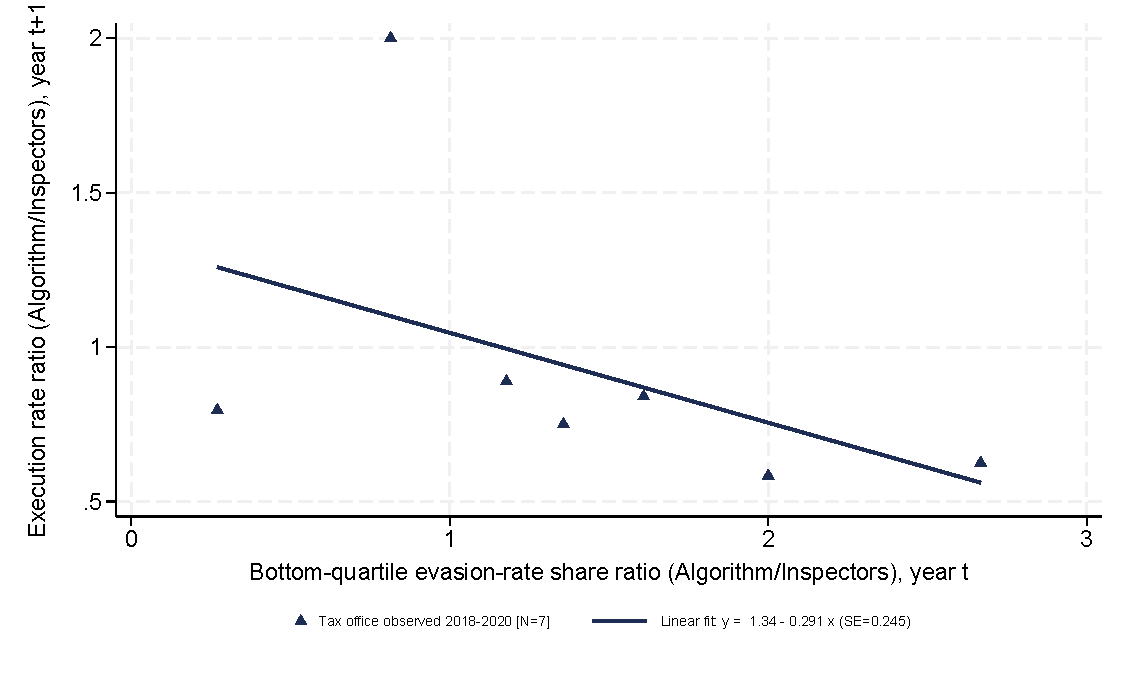
\includegraphics[width=0.5\linewidth]{Output/scatter_share_botq_er_relIns_Algorithm_2018_2019_full.pdf} &
    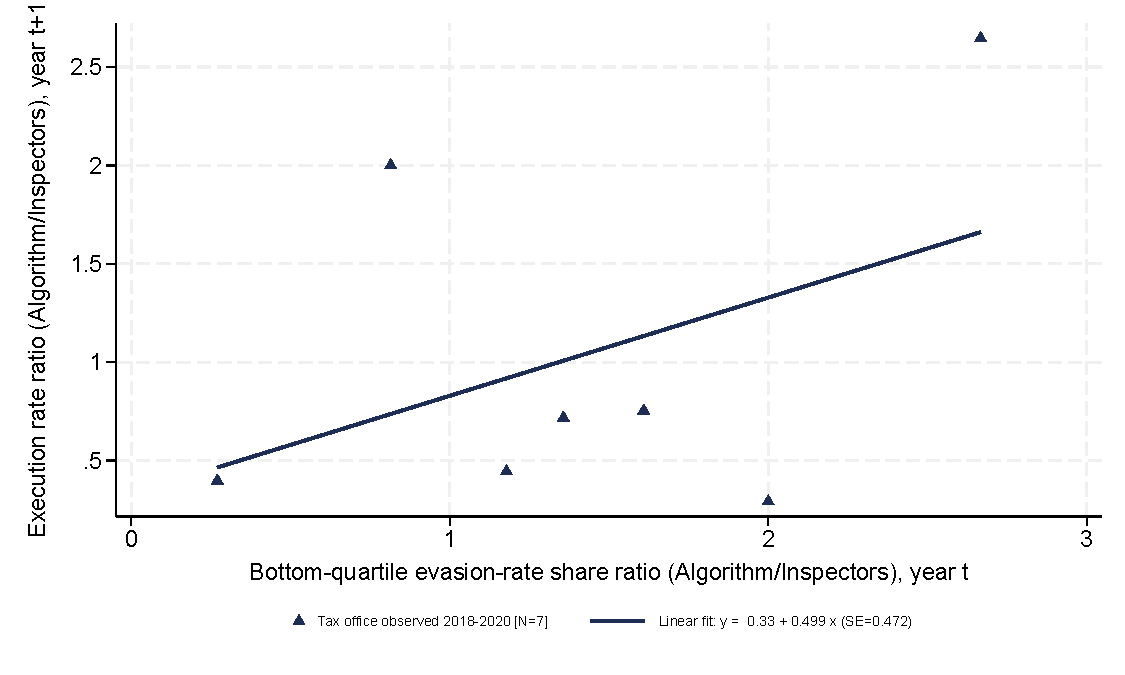
\includegraphics[width=0.5\linewidth]{Output/scatter_share_botq_er_relIns_Algorithm_2018_avg_full.pdf} \\
    \end{tabular}
    \begin{tablenotes}
    \footnotesize \item Notes: The figure relates office-level exposure in year \(t\) to low-yield algorithm-selected audits, measured relative to inspector-selected audits, to the relative algorithm execution rate in \(t+1\) (Algorithm/Inspectors). The sample is selected full audits only, excluding safety cases, aggregated at the tax office-year level. Evasion rate is defined for executed audits as \(\text{evasionvalue}/(\text{evasionvalue}+\text{meanturnover})\), where \(\text{meanturnover}\) is the row mean of available turnover variables. Low-yield measures are: (A) share of void audits, (B) share below the median evasion-rate cutoff, and (C) share in the bottom quartile of the evasion-rate distribution. Median and quartile cutoffs are computed within selection-year \(\times\) selection-group cells (algorithm/random pooled together versus inspectors). Shares use method-specific executed counts as denominators. Relative measures are \(\text{share}_{k,\text{Algorithm}}/\text{share}_{k,\text{Inspectors}}\) for \(k\in\{\text{void},\text{below-median ER},\text{bottom-quartile ER}\}\), and \(\text{exec}_{\text{Algorithm}}/\text{exec}_{\text{Inspectors}}\) for execution rates (\(\text{exec}=\text{executed}/\text{assigned}\)). Ratios are set to missing when inspector shares are zero, and also when method-specific denominators are zero (executed counts for share ratios; assigned counts for execution ratios). The second column compares 2018 with the office-level row mean of 2019 and 2020. Points and fitted lines are unweighted.
    \end{tablenotes}
\end{figure}
